\newpage
\section{Desarrollo}

\hspace{1mm} De acuerdo con los requerimientos solicitados, aproximaremos las funciones de atenuación utilizando Matlab.

\hspace{1mm} Requerimientos:
\begin{itemize}
	\item Banda de paso $800Hz - 1250Hz$, atenuación máxima 0.25dB.
	\item Banda de rechazo $<1200Hz$ y $>5000Hz$, atenuación mínima 30dB.
\end{itemize}

\subsection{Código de Matlab}

\textbf{Parámetros de entrada:}
\begin{verbatim}
	>> %% Parametros de Entrada
	fp=[800 1250]; %Banda de Paso [Hz]
	fs=[200 5000]; %Banda de Rechazo [Hz]
	Wp=2*pi*fp; %Banda de Paso [rad/s]
	Ws=2*pi*fs; %Banda de Rechazo [rad/s]
	Ap=0.25; %Atenuacion maxima en Banda de Paso [dB]
	As=30; %Atenuacion minima en Banda de Rechazo [dB]
\end{verbatim}
\textbf{Cálculo de la FT:}
\begin{verbatim}
	>> %% Calculo de FT
	[n,Wp]=cheb1ord(Wp,Ws,Ap,As,'s');
	[num,den]=cheby1(n,Ap,Wp,'s');
	Filtro=tf(num,den) %Funcion de transferencia calculada
	[sos,g] = tf2sos(num,den); %Descomponemos en bicuadrativas
	%Implementacion como PasaAlto/PasaBajo
	PasaBajo=tf(2*g*sos(1,1:3),sos(1,4:6))
	PasaAlto=tf(1/2*sos(2,1:3),sos(2,4:6))
\end{verbatim}

\textbf{Esto nos devolverá el filtro correspondiente mediante polinomios de Chebychev}

\begin{verbatim}
	Filtro =
	
	1.642e07 s^2
	--------------------------------------------------------------------------------
	s^4 + 5080 s^3 + 9.586e07 s^2 + 2.006e11 s + 1.559e15
	
	Continuous-time transfer function.
\end{verbatim}

\newpage

\textbf{Y tambien su descomposición en dos filtros, Pasa Bajo y Pasa Alto}

\begin{verbatim}
	PasaBajo =
	
	1.642e07
	----------------------------------
	s^2 + 3184 s + 6.632e07
	
	Continuous-time transfer function.
	
	
	PasaAlto =
	
	s^2
	---------------------------------
	s^2 + 1896 s + 2.35e07
	
	Continuous-time transfer function.
\end{verbatim}

\hspace{1mm} Si graficamos, podremos observar el comportamiento de ambos filtros por separado, junto con la conexión de ambos en cascada.\\


\textbf{Ingresamos el siguiente código:}

\begin{verbatim}
	>> %% Graficos
	figure;
	hold on;
	%Especificaciones Filtro
	plot([fs(1)/10 fs(1) fs(1)],[-As -As -Ap],'Color','r','LineWidth',3);
	plot([fs(2) fs(2) fs(2)*10],[-Ap -As -As],'Color','r','LineWidth',3);
	plot([fp(1) fp(1) fp(2) fp(2)],[-As -Ap -Ap -As],'Color','g','LineWidth',3);
	
	
	>> %Filtro
	h = bodeplot(Filtro);
	p = getoptions(h);
	p.PhaseVisible='off';
	p.FreqUnits='Hz';
	p.Grid='on';
	setoptions(h,p);
	bode(PasaBajo);
	bode(PasaAlto);
\end{verbatim}

\begin{figure}[H]
    \centering
    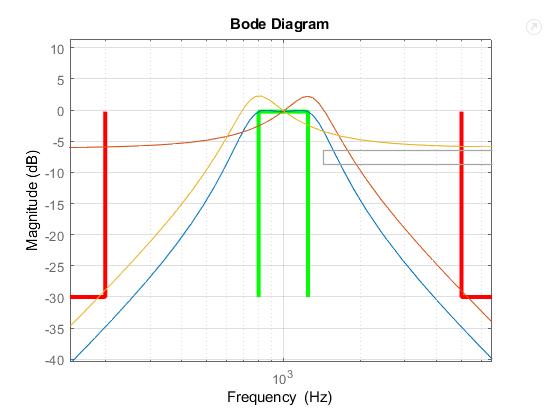
\includegraphics[width=0.8\linewidth]{figuras/Bode.PNG}
    \caption{Diagrama de Bode}
\end{figure}

\hspace{1mm} Siendo el filtro pasa bajos en naranja, pasa altos en amarillo y el filtro total en celeste.
Se cumplen las condiciones de la banda de paso, marcada en verde y las bandas de rechazo marcadas en rojo.\newline

\hspace{1mm} Usando topologías de realimentación positiva Sallen and Key, vamos a sintetizar los filtros requeridos. 

\subsubsection{Filtro Pasabajos}
\begin{verbatim}
	PasaBajo =
	
	1.642e07
	----------------------------------
	s^2 + 3184 s + 6.632e07
\end{verbatim}

\begin{figure}[H]
    \centering
    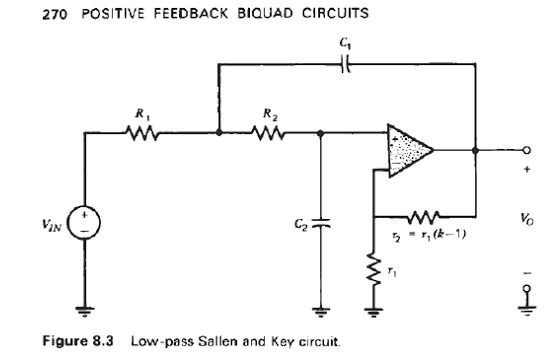
\includegraphics[width=0.75\linewidth]{figuras/Circuito_sallen&key_pasabajos.PNG}
    \caption{Circuito Sallen and Key pasabajos}
    \label{fig:enter-label}
\end{figure}

\hspace{1mm} A partir de los nodos de la red RC planteamos un sistema de ecuaciones:
\begin{center}
	$(V_x - V_i) \cdot \frac{1}{R_1} + (V_x - V_o) \cdot sC_1 + (V_x - V^+) \cdot \frac{1}{R_2} = 0$ \\
	$(V^+ - V_x) \cdot \frac{1}{R_2} + (V^+) \cdot sC_2 = 0 $\\
\end{center}
\hspace{1mm} Operando podemos obtener:

\begin{center}
$V^+ = \frac{N}{D} = \frac{V_i \cdot \frac{S}{R1\cdot R_2 \cdot C_1\cdot C_2} + V_o \cdot \frac{S}{R_2 \cdot C_2}}{\frac{1}{R_1 \cdot R_2 \cdot C_1 \cdot C_2} + S \cdot (\frac{1}{R_1 \cdot C_1}+ \frac{1}{R_2 \cdot C_1}+ \frac{1}{R_2 \cdot C_2})+ S^2}$ \\

$T_{ff} = \frac{N_{ff}}{D} = (\frac{V_+}{V_i})_{V0=0} = \frac{\frac{1}{R_1 \cdot R_2 \cdot C_1 \cdot C_2 }}{D}$ \\ 
$T_{fb} = \frac{N_{fb}}{D} = (\frac{V_+}{V_0})_{Vi=0} = \frac{\frac{S}{R_2 \cdot C_2 }}{D}$ \\
\end{center}
\text{Entonces:} \\
\begin{center}
$\frac{V_0}{V_i} = \frac{k \cdot N_{ff}}{D - k \cdot N_{fb}} =  \frac{\frac{k}{R_1 \cdot R_2 \cdot C_1 \cdot C_2}}{S^2+S \cdot \left(\frac{1}{R_1 \cdot C_1} + \frac{1}{R_2 \cdot C_1} + \frac{1}{R_2 \cdot C_2} - \frac{k}{R_2 \cdot C_2}\right) }$

\end{center}
Donde $k = \frac{r_2+r_1}{r_1}$ \\
\hspace{1mm} Ahora igualamos a la FT requerida: \\
 \begin{center}
 $\frac{1}{R_1 \cdot R_2 \cdot C_1 \cdot C_2}$ = 6.632e07 \\
 $\frac{k}{R_1 \cdot R_2 \cdot C_1 \cdot C_2}$ = 1.642e07 \\
 $\frac{1}{R_1 \cdot C_1} + \frac{1}{R_2 \cdot C_1} + \frac{1}{R_2 \cdot C_2} - \frac{k}{R_2 \cdot C_2} = 3184 $ 
\end{center}
\begin{flushleft}
	Estableceremos: \\
	$ C_1 = C_2 = 0.1 uF $\\
	$ R_1 = R_2 = R $ \\
\end{flushleft} 

\hspace{1mm}Resolviendo las ecuaciones anteriores podemos obtener:\\
R = 1228 Ohm \\
k = 2.6 \\
\hspace{1mm} Por lo tanto: \\
\begin{center}
 $\frac{k}{R_1 \cdot R_2 \cdot C_1 \cdot C_2}$ = $172.41 \cdot 10^6 \neq 1.642e07$ \\
\end{center}

\hspace{1mm} Como esta ganancia es mayor a la requerida en las especificaciones del circuito, planteamos un divisor resistivo en la entrada del mismo para que atenúe.\\


\begin{figure} [H]
    \centering
    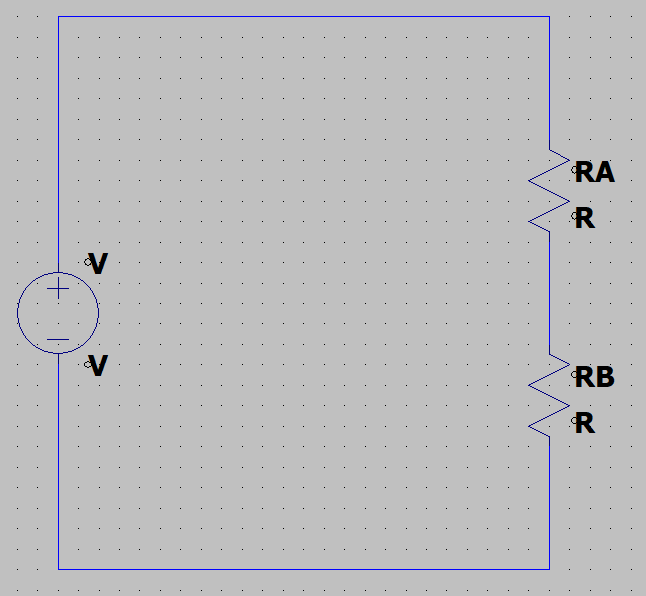
\includegraphics[width=0.75\linewidth]{figuras/DivisorResistivo.PNG}
    \caption{Divisor Resistivo}
\end{figure}

\[
\alpha = \frac{R_A}{R_A + R_B} = \frac{1.642 \times 10^7}{172.41 \times 10^6} = 0.0952
\]

\hspace{1mm} Debemos mantener \( R_1 = R_A//R_B \)

\[
R_A = \frac{R_1}{\alpha} = 12899 \, \Omega
\]
\[
R_B = \frac{\alpha R_A}{1-\alpha} = 1357 \, \Omega
\]

\hspace{1mm} Y para

\[
k = \frac{(R_2 + R_1)}{R_1} = 2.6
\]

\hspace{1mm} Haciendo \( R_1 = 10 \, \text{k} \Omega \)

\( R_2 = 16 \, \text{k} \Omega \)

\subsubsection{Filtro Pasa Altos} 

\text{PasaAlto} = \(\frac{s^2}{s^2 + 1896s + 2.35 \times 10^7}\) \\

\begin{figure}[H]
    \centering
    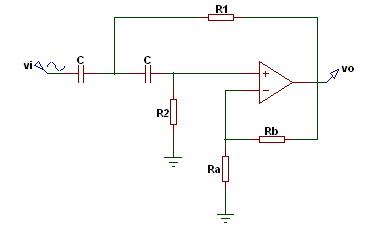
\includegraphics[width=0.75\linewidth]{figuras/filtropasaaltosgen.PNG}
    \caption{Filtro Pasa Alto}
\end{figure}
\hspace{1mm} Planteamos el sistema de ecuaciones:

\[
(V_x - V_i)sC_1 + (V_x - V_o)\frac{1}{R_1} + (V_x - V_+)sC_2 = 0
\]

\[
(V_+ - V_x)sC_2 + (V_+)\frac{1}{R_2} = 0
\]

\textbf{Resolviéndolo obtenemos:}

\[
V_+ = \frac{N}{D} = \frac{V_i s^2 + V_o \cdot \frac{s}{R_{IC1}}}{\frac{1}{R_1 R_2 C_1 C_2} + s \left(\frac{1}{R_{IC1}} + \frac{1}{R_{2C1}} + \frac{1}{R_{2C2}}\right) + s^2}
\]

\[
T_{ff} = \frac{N_{ff}}{D} = \left(\frac{V_+}{V_i}\right)_{V_o=0} = \frac{s^2}{D}
\]

\[
T_{fb} = \frac{N_{fb}}{D} = \left(\frac{V_+}{V_o}\right)_{V_i=0} = \frac{\frac{s}{R_{IC1}}}{D}
\]


\hspace{1mm} Entonces:

\[\frac{V_o}{V_i} = \frac{kNff}{D - kNfb} = \frac{k s^2}{s^2 + s \left( \frac{1}{R_1 C_1} + \frac{1}{R_2 C_1} + \frac{1}{R_2 C_2} + \frac{k}{R_1 C_1} \right) + \frac{1}{R_1 R_2 C_1 C_2}}\]


\hspace{1mm} Siendo \( k = \frac{(R_a + R_b)}{R_a} \) 
\bigskip
\newline
 Igualando a la FT requerida obtenemos:

\[
\frac{1}{R_{\text{1}} R_{\text{2}} C_1 C_2} = 2.35 \times 10^7
\]

\[
k \cdot s^2 = s^2
\]

\[
\frac{1}{R_1 C_1} + \frac{1}{R_2 C_1} + \frac{1}{R_2 C_2} - \frac{k}{R_1 C_1} = 1896
\]

\hspace {1mm}Establecemos:

\begin{itemize}
    \item \( C_1 = C_2 = 0.1 \, \mu \text{F} \)
    \item \( k = 1 \)
\end{itemize}

\hspace{1mm}Y resolviendo las ecuaciones anteriores obtenemos:

\( R_2 = 10548 \, \Omega \)

\( R_1 = 403 \, \Omega \)

\newpage

\section{Simulaciones}

\subsection{Filtro Pasa Bajo}

\begin{figure}[H]
    \centering
    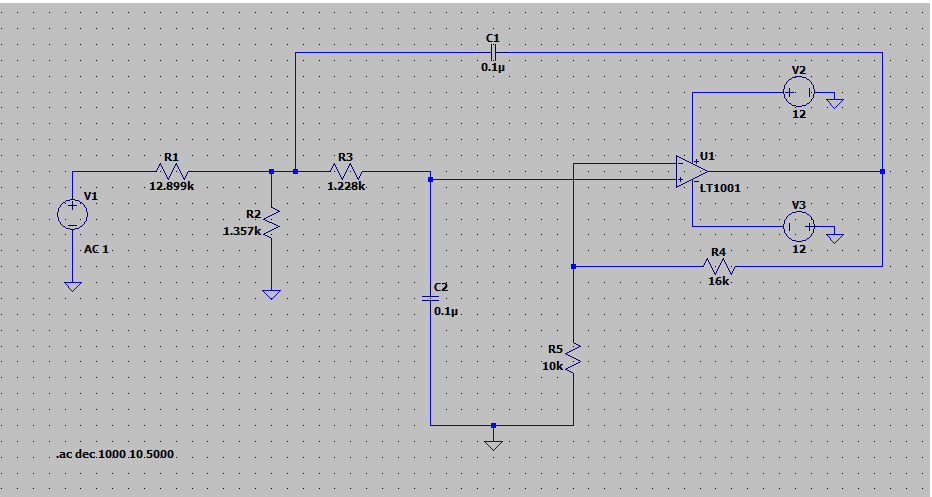
\includegraphics[width=1.0\linewidth]{figuras/Filtro pasa bajo (circ).png}
    \caption{Circuito filtro Pasa Bajo}
\end{figure}

\begin{figure}[H]
    \centering
    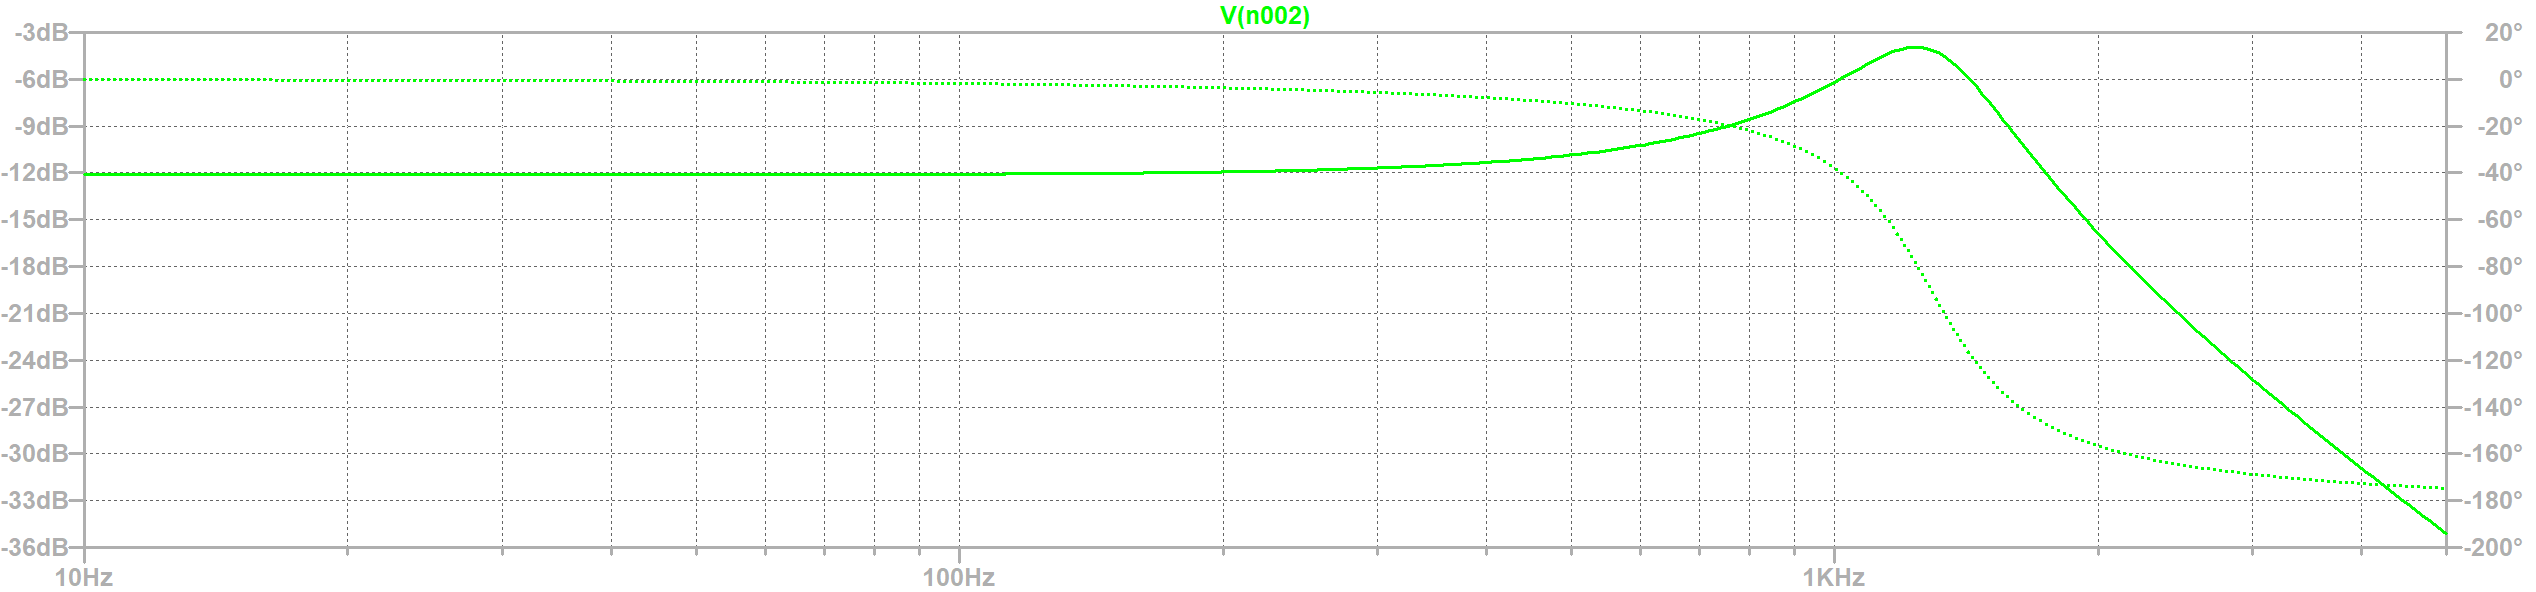
\includegraphics[width=1.0\linewidth]{figuras/filtro pasa bajo (diag).png}
    \caption{Bode filtro Pasa Bajo}
\end{figure}

\newpage
\subsection{Filtro Pasa Alto}

\begin{figure}[H]
    \centering
    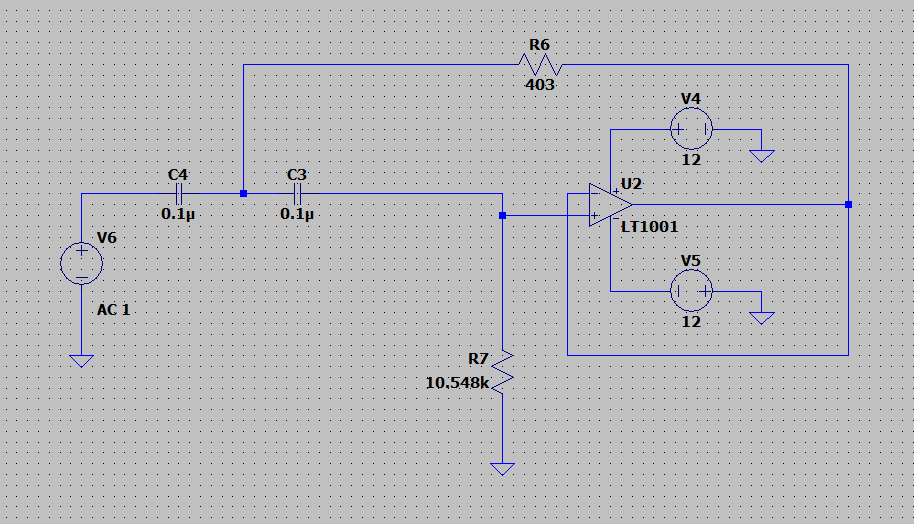
\includegraphics[width=1.0\linewidth]{figuras/filtro pasa altos sim.PNG}
    \caption{Circuito Filtro Pasa Alto}
\end{figure}

\begin{figure}[H]
    \centering
    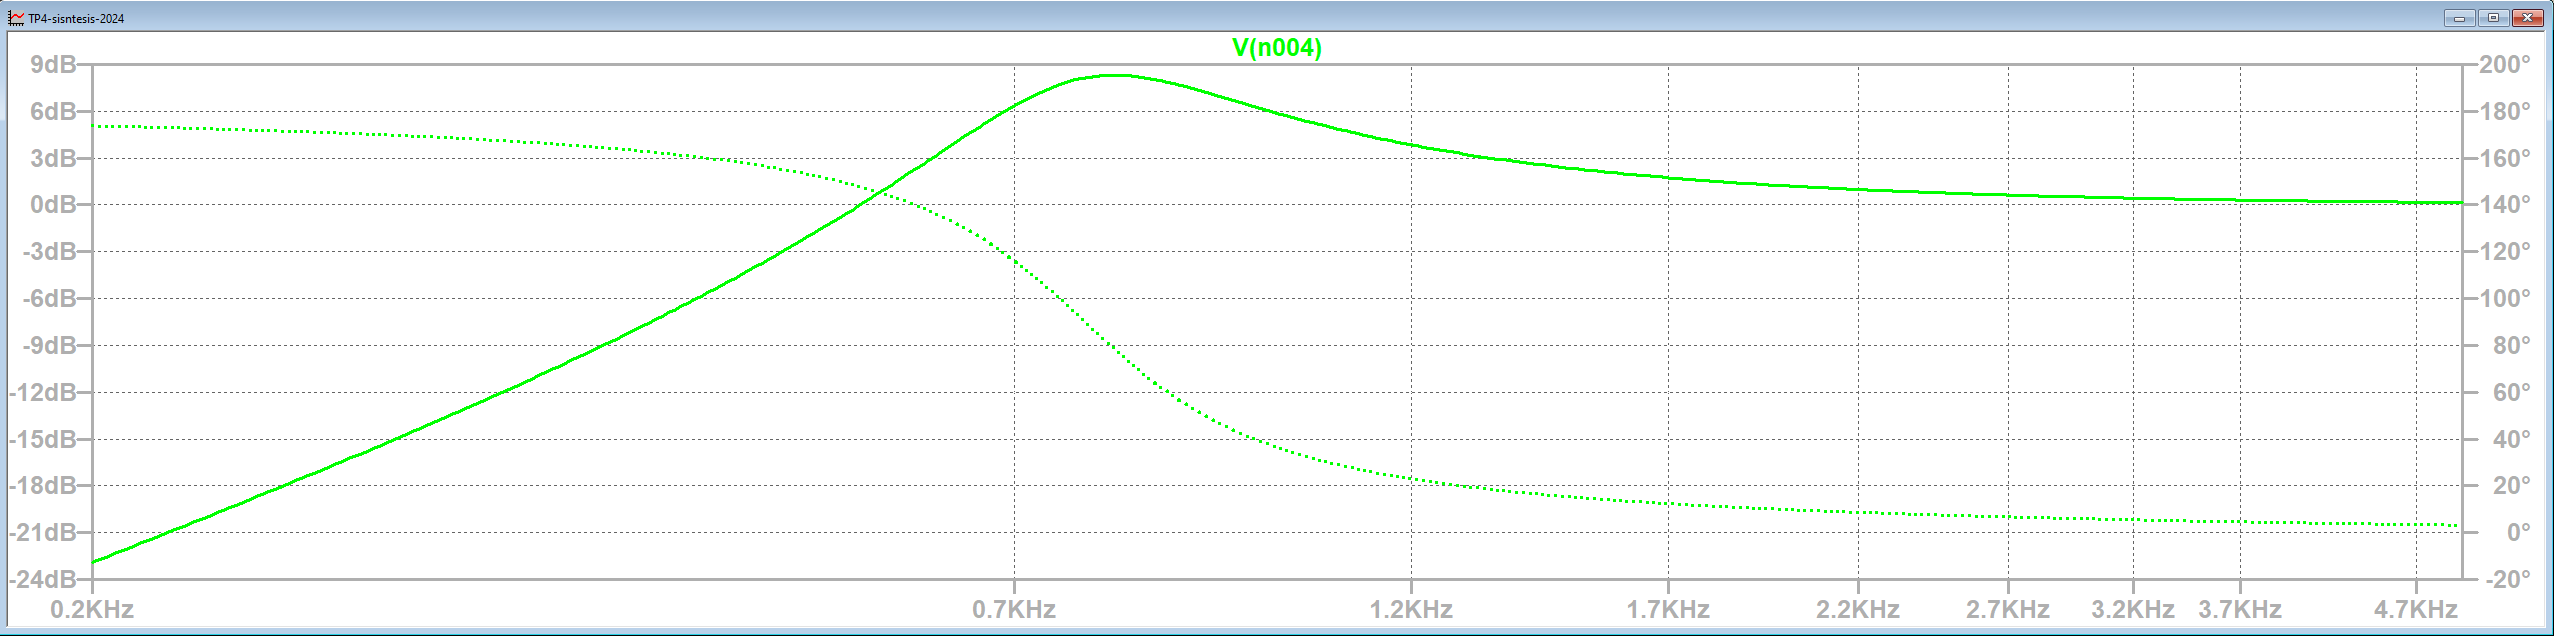
\includegraphics[width=1\linewidth]{figuras/filtro pasa altos circ.PNG}
    \caption{Bode Filtro Pasa Alto}
\end{figure}

\newpage

\subsection{Filtro completo Pasa Banda}

\begin{figure}[H]
    \centering
    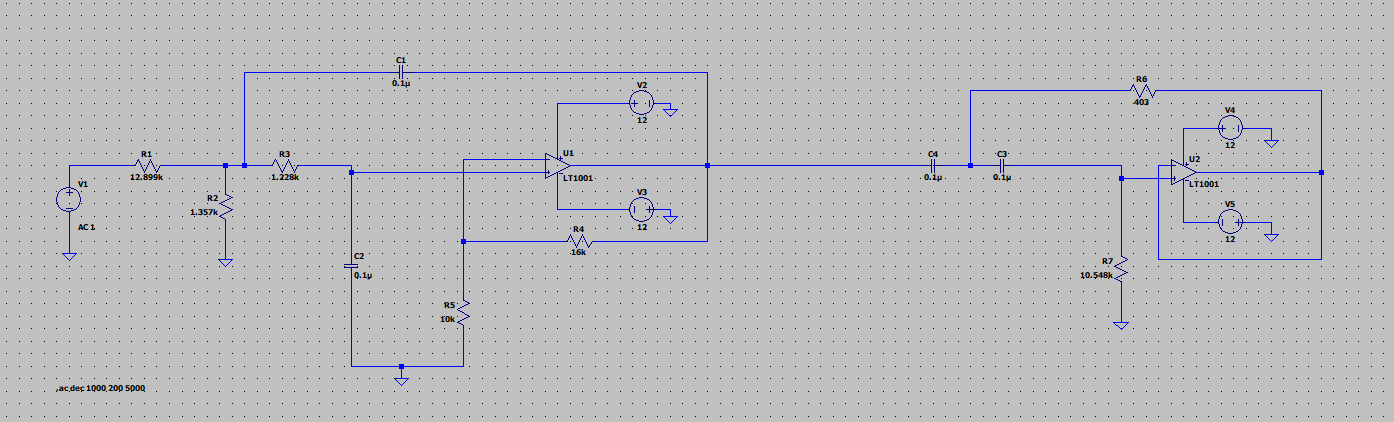
\includegraphics[width=1\linewidth]{figuras/filtro completo circ.PNG}
    \caption{Circuito Filtro Pasa Banda}
\end{figure}

\begin{figure}[H]
    \centering
    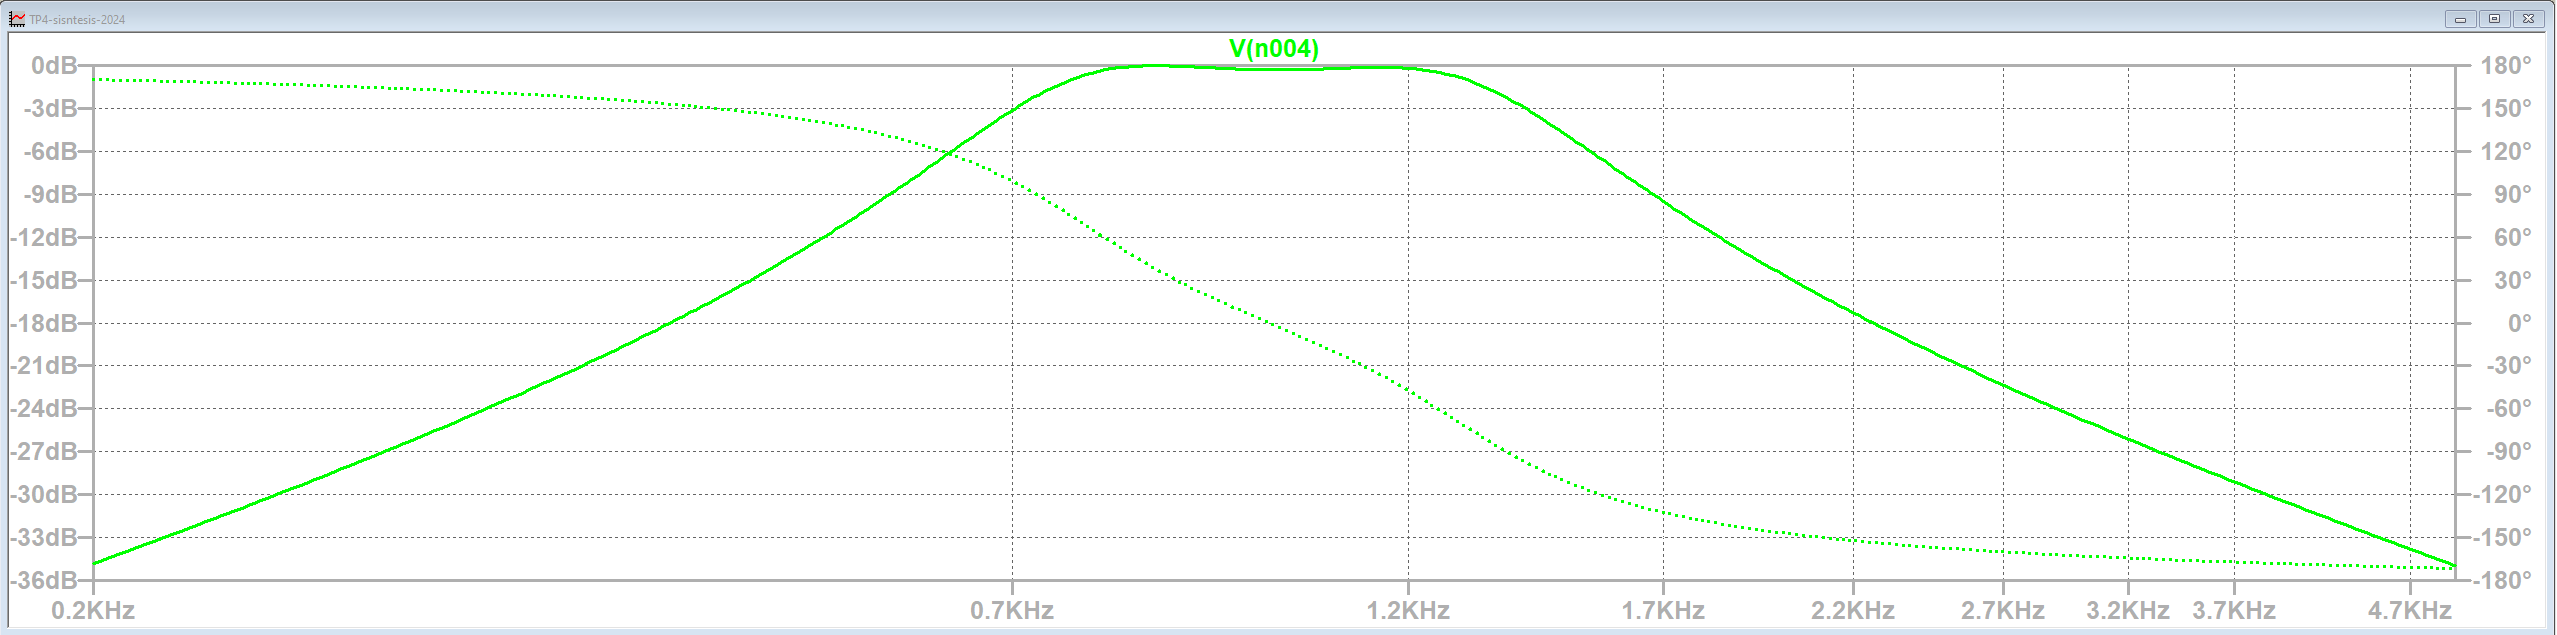
\includegraphics[width=1\linewidth]{figuras/filtro completo sim.PNG}
    \caption{Bode Filtro Pasa Banda}
\end{figure}
\text{Utilizando los cursores para mayor detalle:} 
\begin{figure}[H]
    \centering
    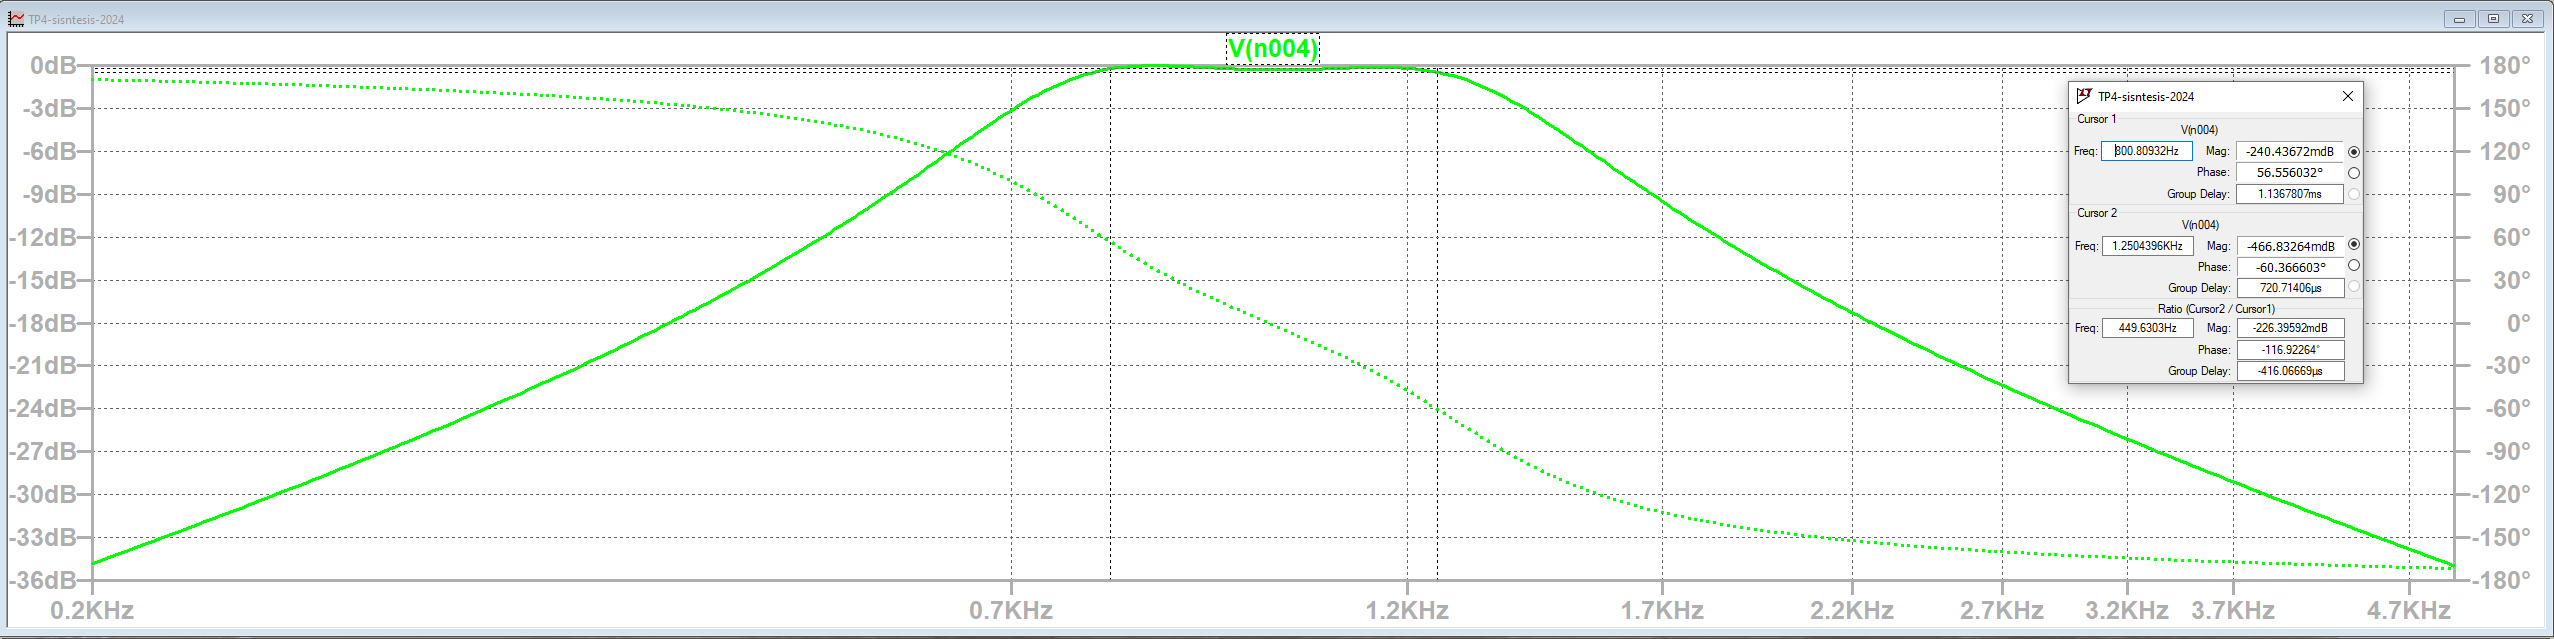
\includegraphics[width=1\linewidth]{figuras/filtro completo cursores.PNG}
    \caption{Cursor 1}
\end{figure}
\begin{figure}[H]
    \centering
    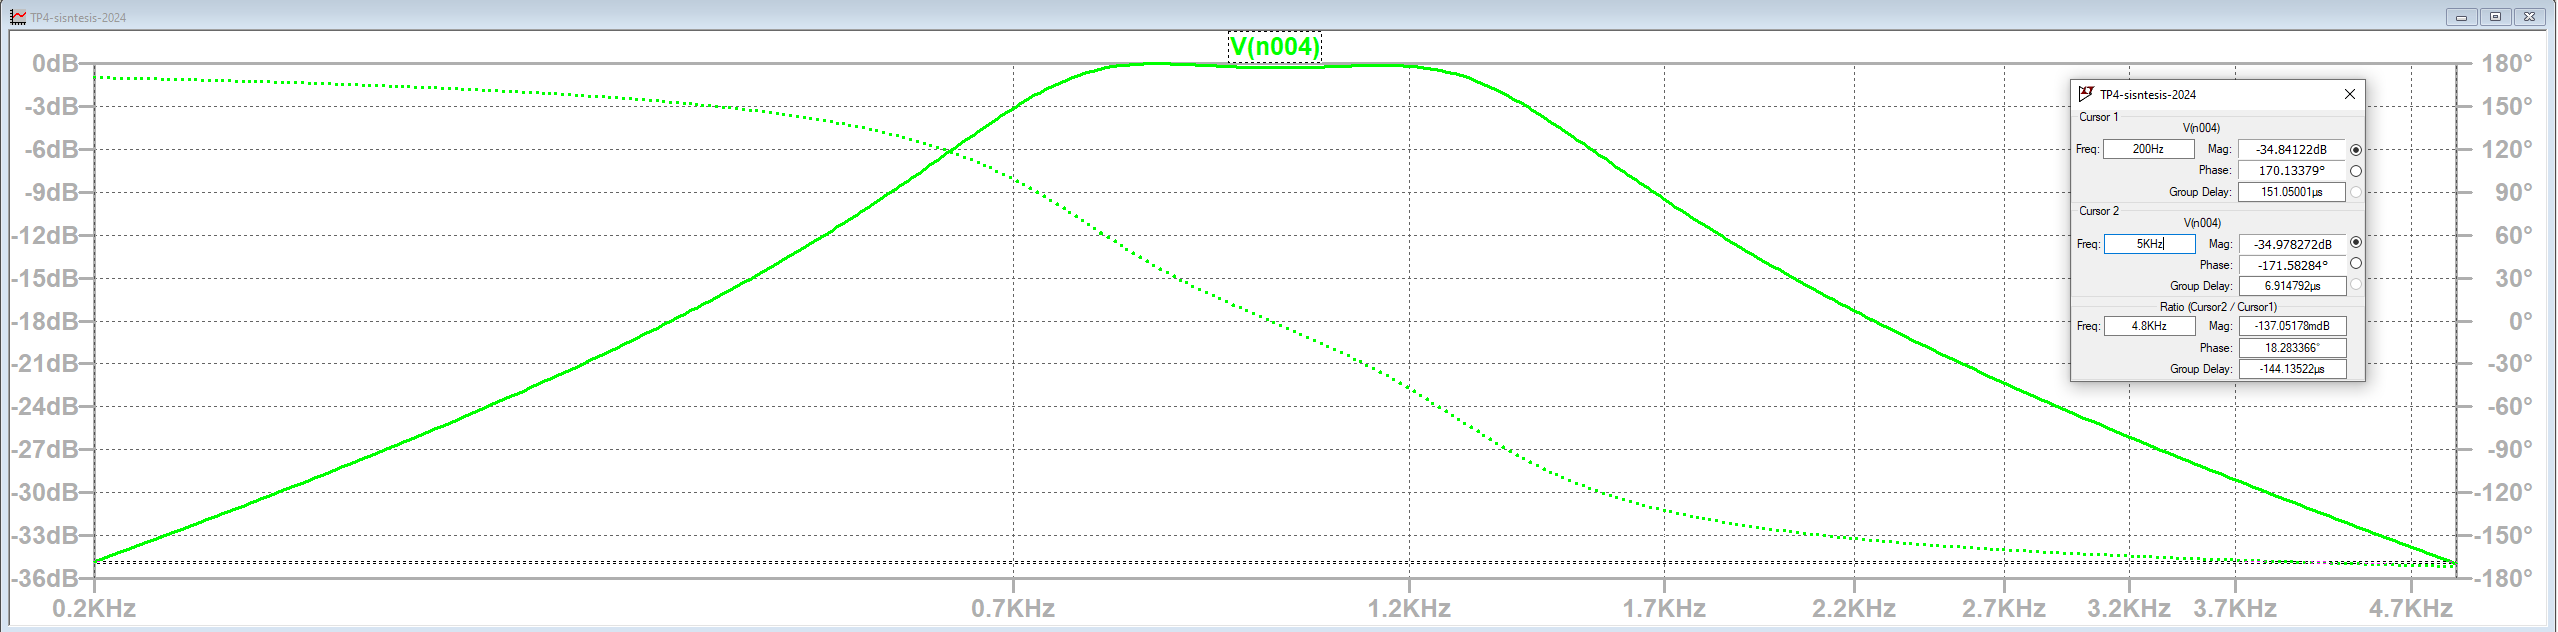
\includegraphics[width=1\linewidth]{figuras/circuito completo cursor 2.PNG}
    \caption{Cursor 2}
\end{figure}

\hspace{1mm} Pueden observarse las atenuaciones en las frecuencias de nuestro interés: 

\begin{itemize}
\item 800 Hz : -0.240 dB
\item 1250 Hz : -0.466 dB
\item 200 Hz : -34.84 dB
\item 500 Hz : -34.97 dB
\end{itemize}
\hspace{1mm} Las cuales cumplen con los requerimientos del circuito.

\newpage

\section{Cálculo de la sensibilidad}
\hspace{1mm} Para el cálculo de la sensibilidad de la frecuencia del polo (\(\omega_p\)) y el ancho de banda (\(\omega_p / Q_p\)) simplemente tomamos de la ecuación principal la deducción de \(\omega_p\) la cual es:

\[\omega_p = \sqrt{\frac{1}{R_1 \cdot R_2 \cdot C_1 \cdot C_2}} = \frac{1}{\sqrt{R_1 \cdot R_2 \cdot C_1 \cdot C_2}}\]

\hspace{1mm}Y para el ancho de banda:

\[\frac{\omega_p}{Q_p} = \frac{1}{R_1 C_1} + \frac{1}{R_2 C_1} + \frac{1}{R_2 C_2} - \frac{k}{R_1 C_1}\]

\hspace{1mm}Definimos entonces la sensibilidad según los resistores:

\[
\mathcal{S}\left(\frac{\omega_p}{R}\right) = \frac{\frac{\Delta \omega_p}{\omega_p}}{\frac{\Delta R}{R}} = \frac{R}{\omega_p} \cdot \frac{\partial \omega_p}{\partial R}
\]

\[
\mathcal{S}\left(\frac{\omega_p}{C}\right) = \frac{\frac{\Delta \omega_p}{\omega_p}}{\frac{\Delta C}{C}} = \frac{C}{\omega_p} \cdot \frac{\partial \omega_p}{\partial C}
\]

\[
\mathcal{S}\left(\frac{\frac{\omega_p}{Q_p}}{R}\right) = \frac{\frac{\Delta \omega_p}{\omega_p}}{\frac{\Delta R}{R}} = \frac{R}{\frac{\omega_p}{Q_p}} \cdot \frac{\partial \left(\frac{\omega_p}{Q_p}\right)}{\partial R}
\]

\[
\mathcal{S}\left(\frac{\frac{\omega_p}{Q_p}}{C}\right) = \frac{\frac{\Delta \omega_p}{\omega_p}}{\frac{\Delta C}{C}} = \frac{C}{\frac{\omega_p}{Q_p}} \cdot \frac{\partial \left(\frac{\omega_p}{Q_p}\right)}{\partial C}
\]
 \hspace{1mm} Plantearemos una tabla con las sensibilidades correspondientes tomando en cuenta la peor desviación con una tolerancia del 10\% de cada componente:

\renewcommand{\arraystretch}{1.5}
\begin{table}[H]
\centering
\begin{tabular}{|>{\columncolor[HTML]{B3D9FF}}c|>{\centering\arraybackslash}m{2.5cm}|>{\centering\arraybackslash}m{2.5cm}|>{\centering\arraybackslash}m{3cm}|>{\centering\arraybackslash}m{2.5cm}|}
\hline
\rowcolor[HTML]{B3D9FF} 
     & $\omega_p$ & $\frac{P}{10\%}$ & $\frac{\omega_p}{Q_p}$ & $\frac{P}{10\%}$ \\ \hline
\cellcolor[HTML]{B3D9FF} R1 & $-\frac{1}{2}$ & 5\% & $\frac{-1}{4-K}$ & 18\% \\ \hline
\cellcolor[HTML]{B3D9FF} R2 & $-\frac{1}{2}$ & 5\% & $\frac{-(K-2)}{4-K}$ & 26\% \\ \hline
\cellcolor[HTML]{B3D9FF} C1 & $-\frac{1}{2}$ & 5\% & $\frac{-(K-3)}{4-K}$ & 8\% \\ \hline
\cellcolor[HTML]{B3D9FF} C2 & $-\frac{1}{2}$ & 5\% & $\frac{-1}{4-K}$ & 18\% \\ \hline
\cellcolor[HTML]{B3D9FF} TOTAL & -2 & 20\% & -7 & 70\% \\ \hline
\end{tabular}
\end{table}

\newpage

\section{Análisis de Montecarlo de los componentes}
\hspace{1mm} Para realizar este análisis se varían los valores de los componentes pasivos del circuito de acuerdo a su tolerancia y se toma distribución normal de estos mismo. Se plantea una distribución estadistica del posible valor de la frecuencia del polo de cada etapa ($\omega_p$) , o del ancho de banda correspondiente ($\omega_p$/$Q_p$).

\begin{figure}[H]
    \centering
    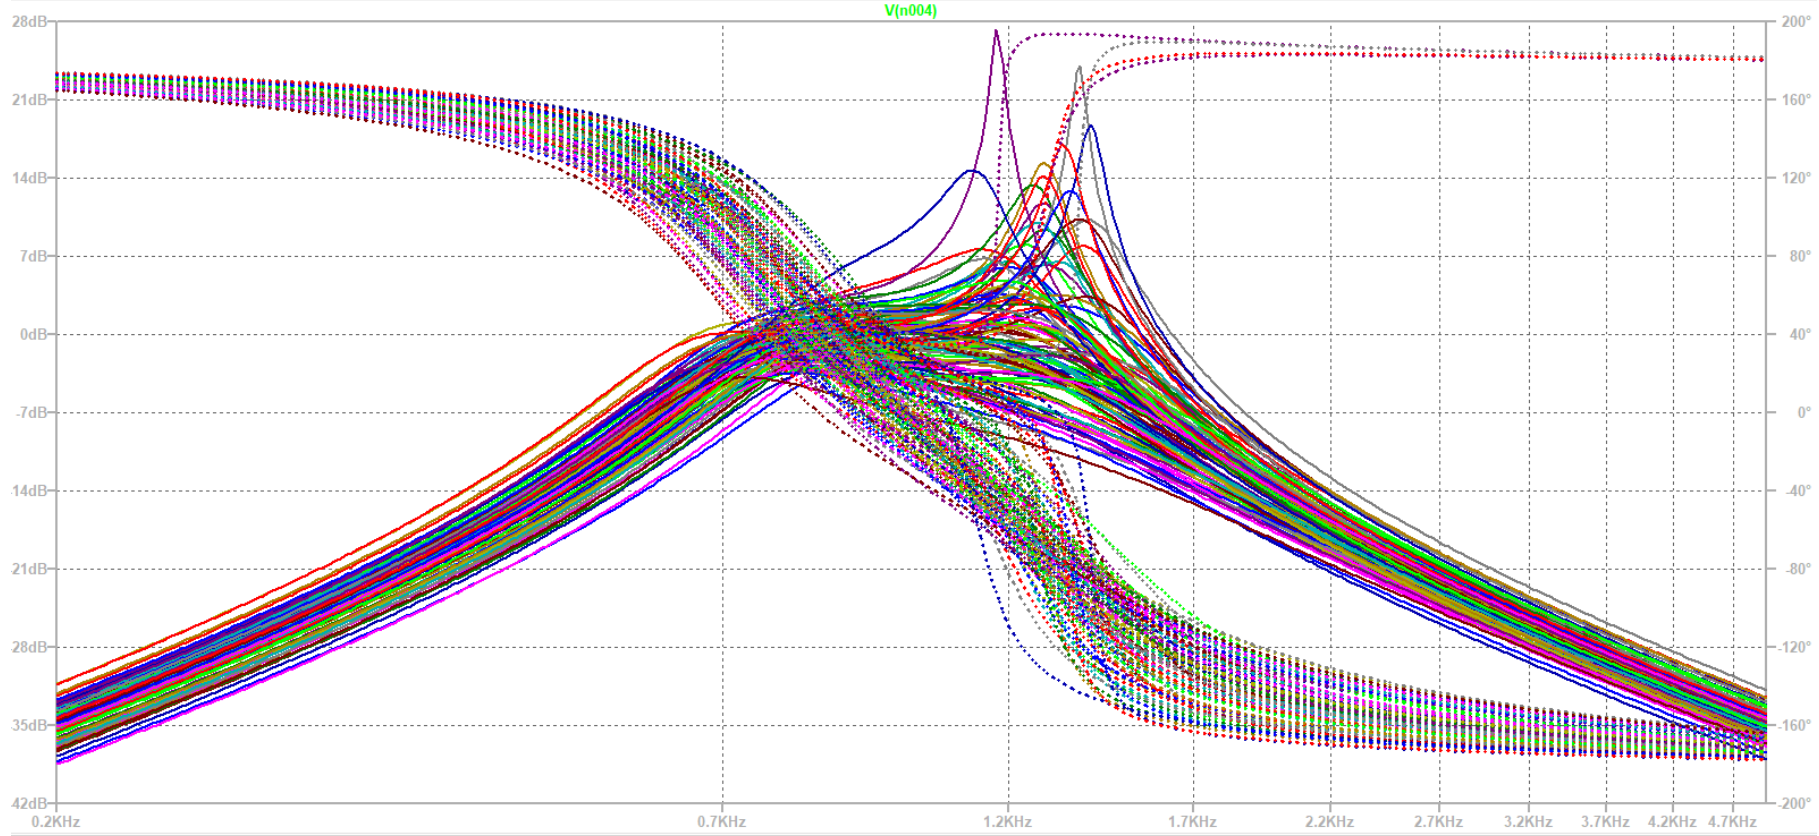
\includegraphics[width=1.0\linewidth]{figuras/AnalisisMontecarlo.PNG}
    \caption{Análisis de Montecarlo}
\end{figure}

\newpage

\section{Conclusiones}
\hspace{1mm} La implementación del circuito nos permitió profundizar en la síntesis y diseño de un filtro pasabanda, así como en las variaciones que los valores de los componentes pueden ejercer sobre el desempeño del sistema y su sensibilidad respecto a cada uno de estos componentes. Además, nos familiarizamos con el entorno de simulación, en el cual pudimos verificar el funcionamiento correcto del diseño realizado.

\hspace{1mm} Observamos la utilidad de realizar dos diseños más sencillos, como un filtro pasa bajos y un filtro pasa altos, para lograr un filtro pasabanda altamente eficaz.


